%!TEX root = ../main.tex

\chapter{Introducción}
\label{intro}

En las últimas dos décadas distintas técnicas de ingeniería reversa del aprendizaje en humanos han inspirado con éxito variados algoritmos de inteligencia artificial~\cite{russell2002artificial}. Los avances recientes en las técnicas de aprendizaje profundo han logrado resultados notables en numerosos dominios como el reconocimiento visual de objetos, el reconocimiento automático del habla, la búsqueda de respuestas y las traducciones automáticas aprovechando los grandes volúmenes de datos disponibles~\cite{lecun2015deep}. En la mayoría de estos enfoques, el resultado y el objeto del proceso de aprendizaje es una función estadística de reconocimiento de patrones específicos en los datos. Sin embargo, en muchas situaciones, el aprendizaje humano implica la construcción de modelos estructurados de conocimiento abstracto, los cuáles son construidos incluso a partir de la exposición a muy pocos datos, y este tipo de sistemas no han sido capaces de imitar esa habilidad~\cite{lake2017building}.

¿Cómo pueden las personas adquirir un vasto universo de conceptos con muy poca exposición aparente? Una posible solución a este enigma, conocida como el problema de Platón~\cite{chomsky1986knowledge, chomsky2006cognitive}, surge del aprendizaje automático probabilístico. Este enfoque está arrojando algo de luz sobre cómo los humanos pueden construir modelos y abstracciones bajo incertidumbre y a partir de datos escasos~\cite{tenenbaum2011grow,ghahramani2015probabilistic}, y está renovando la hipótesis de Jerry Fodor que afirma que el pensamiento toma forma en una especie de lenguaje mental del pensamiento (\lot, por sus siglas en inglés) compuesto por un conjunto limitado de símbolos atómicos que se pueden combinar para formar estructuras más complejas siguiendo reglas combinatorias~\cite{fodor1975language}.

Nuestra investigación se suscribe a una de las líneas actuales del aprendizaje automático probabilístico conocida como lenguajes del pensamiento probabilísticos~\cite{goodman2014concepts}, un esquema general para expresar modelos probabilísticos y métodos de inferencia sobre lenguajes formales. En nuestro caso, estos lenguajes definen cada uno un lenguaje de programación que, al computarse según su propia semántica, representan conceptos del mundo. Con nuestro trabajo pretendemos mejorar nuestro entendimiento del proceso de aprendizaje a partir de cuerpos ralos de datos y desarrollar nuevos métodos y algoritmos de programación probabilística para replicar esta notable capacidad humana. 


\section{Aportes de esta tesis}

\paragraph{Una teoría de la memoria para secuencias binarias: evidencia de un algoritmo de compresión mental en humanos~\cite{planton2021memory}.} 
La capacidad de la memoria de trabajo se puede mejorar recodificando la información memorizada en forma condensada. En el Capítulo~\ref{chapter:BIN}, ponemos a prueba la teoría de que los adultos humanos codifican secuencias binarias de estímulos en la memoria utilizando un \lot y un algoritmo de compresión recursivo. La teoría predice que la complejidad psicológica de una secuencia dada debería ser proporcional a la longitud de su descripción más corta en el lenguaje propuesto \grambin, que puede capturar cualquier patrón anidado de repeticiones y alternancias usando un número limitado de instrucciones. El lenguaje \grambin es una versión simplificada para el dominio de las secuencias binarias del lenguaje de geometría, \gramgeo, propuesto en~\cite{amalric2017language}. Cinco experimentos examinan la capacidad de la teoría para predecir la memoria de los adultos humanos para una variedad de secuencias auditivas y visuales. Pusimos a prueba la memoria utilizando un paradigma de violación de secuencia en el que los participantes intentaron detectar violaciones ocasionales en una secuencia fija. Tanto las calificaciones de complejidad subjetiva como el rendimiento de detección de violaciones objetivas fueron bien predichas por nuestra medida teórica de complejidad, que resulta ser la complejidad de Kolmogorov para el lenguaje específico de geometría en cadenas binarias, \grambin. Los resultados apoyan la hipótesis de que, más allá de la extracción de conocimiento estadístico, la codificación de secuencias humanas se basa en una compresión interna que utiliza estructuras anidadas similares a las del \lot propuesto.


\paragraph{Validación Bayesiana de producciones gramaticales para el \lot~\cite{romano2018bayesian}.} 
Las propuestas probabilísticas del \lot pueden explicar el aprendizaje en diferentes dominios como una inferencia estadística sobre un espacio de hipótesis estructurado composicionalmente. Si bien los marcos pueden diferir en cómo se puede implementar un \lot computacionalmente, todos comparten la propiedad de que se construyen a partir de un conjunto de símbolos atómicos y reglas mediante las cuales estos símbolos se pueden combinar. En el Capítulo~\ref{chapter:PO} se propone un paso de validación extra para el conjunto de producciones atómicas definidas por el experimentador. Comienza expandiendo la gramática \lot definida para el dominio cognitivo con un conjunto más amplio de producciones arbitrarias y luego usa la inferencia Bayesiana para podar las producciones de los datos experimentales. El resultado permite al investigador validar que la gramática resultante aún coincide con la gramática intuitiva elegida para el dominio. Luego se prueba este método en el lenguaje \gramgeo, un modelo de \lot específico para el aprendizaje de secuencias geométricas propuesto en~\cite{amalric2017language}. Finalmente, a pesar de que \gramgeo no es un lenguaje universal (es decir, Turing completo), mostramos una relación empírica entre la probabilidad de una secuencia y su complejidad, consistente con la relación teórica para los lenguajes universales descrita por el Teorema de codificación de Levin~\cite{levin1974laws}.


\paragraph{Hacia un \lot más flexible: la gramática Bayesiana se actualiza después de cada exposición de conceptos~\cite{tano2020towards}.}
Los enfoques recientes del aprendizaje de conceptos humanos han combinado con éxito el poder de los sistemas de reglas simbólicos e infinitamente productivos y el aprendizaje estadístico para explicar nuestra capacidad de aprender nuevos conceptos a partir de unos pocos ejemplos. El objetivo de la mayoría de estos estudios es revelar el lenguaje subyacente que estructura estas representaciones y proporciona un sustrato general para el pensamiento. Sin embargo, describir un modelo de pensamiento que se fija una vez entrenado va en contra de la extensa literatura que muestra cómo la experiencia da forma al aprendizaje de conceptos. En el Capítulo~\ref{chapter:PRE} se investiga la plasticidad de estos lenguajes descriptivos simbólicos. Se realiza un experimento de aprendizaje de conceptos que demuestra que los seres humanos pueden cambiar muy rápidamente el repertorio de símbolos que utilizan para identificar conceptos, compilando expresiones que se utilizan con frecuencia en nuevos símbolos del lenguaje. El patrón de tiempos de aprendizaje de conceptos es descrito con precisión por un agente Bayesiano que actualiza racionalmente la probabilidad de compilar una nueva expresión de acuerdo con lo útil que ha sido para comprimir conceptos hasta ahora. Al presentar el \lot como un sistema flexible de reglas, también destacamos las dificultades para precisarlo empíricamente.

\paragraph{Un marco lógico para estudiar los sesgos de aprendizaje de conceptos en presencia de múltiples explicaciones~\cite{tano2021framework}.}
Cuando las personas buscan comprender conceptos a partir de un conjunto incompleto de ejemplos y contraejemplos, suele haber una cantidad exponencial de reglas de clasificación que pueden clasificar correctamente los datos observados, según las características de los ejemplos que se utilicen para construir estas reglas. Una aproximación mecanicista del aprendizaje de conceptos humanos debería ayudar a explicar cómo los humanos prefieren algunas reglas por sobre otras cuando hay muchas que pueden usarse para clasificar correctamente los datos observados. En el Capítulo~\ref{chapter:BRM}, se explotan las herramientas de la lógica proposicional para desarrollar un marco experimental --continuando y ampliando aquel desarrollado en el Capítulo~\ref{chapter:PRE}-- que controle las reglas mínimas que son \textit{simultáneamente} consistentes con los ejemplos presentados. Por ejemplo, este marco nos permite presentar a los participantes conceptos consistentes con una disyunción \textit{y también} con una conjunción, dependiendo de qué características se usen para construir la regla. Del mismo modo, nos permite presentar conceptos que son simultáneamente consistentes con dos o más reglas de diferente complejidad y que utilizan diferentes características. Es importante destacar que el marco lógico propuesto controla completamente qué reglas mínimas compiten para explicar los ejemplos y es capaz de recuperar las características utilizadas por el participante para construir la regla de clasificación, sin depender de mecanismos complementarios de seguimiento de la atención (por ejemplo, {\em eye-tracking}). Explotamos el marco estudiado en un experimento con una secuencia de pruebas competitivas como las mencionadas, e ilustramos la aparición de varios efectos de transferencia que sesgan la atención previa de los participantes a conjuntos específicos de características durante el aprendizaje.


\section{Lenguaje del pensamiento}

El objetivo de programar agentes inteligentes y el estudio de la mente humana han creado preguntas compartidas y sinergias comunes entre los campos de la inteligencia artificial y la ciencia cognitiva~\cite{russell2002artificial}. Dentro de estas, la adquisición de conceptos ha resultado un aspecto clave y ampliamente estudiado tanto en la cognición humana como en la inteligencia artificial~\cite{cohen2005handbook, ashby2011human,tenenbaum2011grow}.

Los investigadores han modelado el aprendizaje de clases conceptuales para los objetos principalmente con dos enfoques clásicos: en términos de similitud con un ejemplo genérico o prototipo~\cite{rosch1999principles, nosofsky1986attention, rosch1976structural, rosch1975family} o basándose en una representación simbólica de reglas~\cite{boole1854investigation, fodor1975language, gentner1983structure}.

Los trabajos basados en modelos prototipos proponen que los humanos construyen una representación promedio o protípica para cada clase conceptual y basan la clasificación de un ejemplo en función de la distancia relativa a cada clase~\cite{wilson2001encyclopedia}. Mientras que los enfoques simbólicos sostienen que los pensamientos son representaciones simbólicas en un \textit{lenguaje del pensamiento} (\lot) compuesto por un conjunto limitado de símbolos atómicos que pueden combinarse para formar estructuras nuevas y más complejas siguiendo reglas combinatorias~\cite{fodor1975language,nosofsky1994rule, tenenbaum2011grow, maddox1993comparing}. 

El \lot no es necesariamente único, la forma que adopta se ha modelado de muchas formas diferentes según el dominio del problema: aprendizaje de conceptos numéricos~\cite{piantadosi2012bootstrapping}, aprendizaje de secuencias~\cite{amalric2017language, yildirim2015learning, romano2013language}, aprendizaje de conceptos visuales~\cite{ellis2015unsupervised}, aprendizaje de teorías~\cite{ullman2012theory}, etc. De hecho, en la parte \ref{parte:secuencias} de esta tesis, trabajaremos con dos modelos distintos de \lot: para el dominio de secuencias binarias en el capítulo \ref{chapter:BIN}, y para el dominio de secuencias geométricas en el capítulo~\ref{chapter:PO}.

A pesar de las críticas y objeciones~\cite{blackburn1984spreading,loewer1991meaning,knowles1998language,aydede1997language,wilson2001encyclopedia}, los enfoques simbólicos --en general-- y la hipótesis \lot{ }--en particular-- han ganado una atención renovada con resultados recientes que podrían explicar el proceso de aprendizaje en diferentes dominios como un proceso de inferencia estadística sobre un espacio de hipótesis estructurado y componible~\cite{tenenbaum2011grow,piantadosi2016four}, fusionando de esta manera la expresividad de los lenguajes formales con la flexibilidad y el poder de los mecanismos de inferencia probabilística.

%Las investigaciones indican que --como mínimo-- dos sistemas distintos pueden ser parte de la base del aprendizaje de secuencias\santi{no me quedó claro el hilo conductor. Acá estas hablando de secuencias específicamente pero con los dos enfoques que describiste más arriba? Usás 'aprendizaje estadístico' para referirte a lo que antes llamaste 'enfoque basado en prototipos'?} en el cerebro humano: el aprendizaje estadístico y el aprendizaje basado en reglas~\cite{f4,f67,f85}. Lo que se desconoce es si operan de forma independiente o conjunta, y si alguno es favorecido por sobre el otro en función de la naturaleza de la información a codificar. Argumentamos que cualquier intento por descubrir los mecanismos cognitivos específicos detrás del aprendizaje de reglas en humanos, especialmente en comparación con otras especies, debe tener también en cuenta la contribución de un sistema menos abstracto (sin embargo, poderoso) de predicción basado en las propiedades estadísticas de los eventos. 

Los lenguajes simbólicos pueden describir un vasto conjunto de conceptos a partir de un pequeño conjunto de primitivas y reglas combinatorias. Podemos entenderlo con un ejemplo relativamente simple en el dominio de las formas. Un lenguaje combinatorio similar a Logo~\cite{abelson1974logo} puede combinar símbolos de operaciones como ``mover", ``lápiz arriba", ``lápiz abajo'' o ``rotar" para generar un conjunto infinito de expresiones (o programas) que, cuando se evalúan, pueden trasmitir todo tipo de formas.

Una pregunta natural, sobre la que profundizaremos en la parte \ref{parte:conceptos}, es si las primitivas de un \lot son universales --tanto a través de diferentes individuos como a lo largo del desarrollo-- o si, en cambio, el repertorio semántico de un lenguaje es dinámico y está moldeado por la experiencia. De hecho, es probable que nuestra capacidad para representar automáticamente conceptos de manera sucinta no se deba a un lenguaje eficiente innato en nuestra mente. En cambio, proponemos que esta capacidad surge como un subproducto de nuestro cerebro que aprende rápidamente representaciones eficientes de los conceptos que generalmente encontramos en la vida cotidiana. Examinaremos la hipótesis de que los humanos tienen la capacidad de recombinar rápidamente proposiciones en su \lot, agregando nuevas primitivas a su lenguaje. En otras palabras, ese aprendizaje conduce a un proceso de compilación de rutinas en funciones dentro de el \lot.

En el ejemplo del lenguaje Logo se puede imaginar que si las producciones que dibujan cuadrados son muy frecuentes, sería eficaz dedicar un nuevo símbolo a esta producción. El nuevo símbolo ``cuadrado'' es una construcción jerárquica de {\em segundo orden} de las primitivas de {\em primer orden} del lenguaje. Tiene un costo (el de incrementar el léxico del lenguaje) pero en el nuevo lenguaje, dibujar un cuadrado puede ser instanciado con un programa muy corto (simplemente, {\em cuadrado}) y por lo tanto usa menos memoria. De hecho, un lenguaje de nivel superior nos permite alcanzar un nivel superior de abstracción al liberar la memoria y el poder de procesamiento, haciendo así pensables pensamientos más complejos~\cite{minsky1967computation, murphy1988comprehending}.

La mayor parte del trabajo en la literatura sobre \lot, aunque incluye naturalmente un mecanismo de aprendizaje, tiende a acercarse al \lot como un sistema estable que deben descubrir los experimentadores, que prueban diferentes plantillas candidatas y seleccionan la que mejor se ajusta a los datos después del entrenamiento ~\cite{goodman2008rational, kemp2012exploring, piantadosi2016logical}. Aún así, queda por descubrir cómo las diferentes trayectorias de la experiencia pueden dar forma a la adquisición de manera diferente y pueden cambiar constantemente el repertorio de un \lot después de cada exposición.

Un lenguaje que describe conceptos (como las formas) también proporciona una noción natural de su complejidad~\cite{kolmogorov1968three} y se ha observado que aprendemos conceptos de objetos con más facilidad cuando hay reglas `más simples' que pueden explicar esas agrupaciones~\cite{shepard1961learning, nosofsky1994comparing, rehder2005eyetracking, lewandowsky2011working, feldman2000minimization, blair2003easy, minda2001prototypes}. Un concepto es simple, relativo a ese lenguaje, cuando puede ser descripto por un programa corto. Por el contrario, es complejo cuando todas sus descripciones requieren una secuencia larga de instrucciones. Por ejemplo, en el caso de Logo, un cuadrado se puede codificar simplemente como un bucle de cuatro desplazamientos seguidos de rotaciones de 90 grados. En cambio, describir una cara requerirá de un programa más largo y, por lo tanto, será un concepto más complejo de describir. Sin embargo, este concepto se podría describir de manera más simple en un lenguaje en el que el icono de una cara (o de una nariz, boca, etc.) estuvieran disponibles como primitivas de ese lenguaje. 

De hecho, la correlación entre la dificultad subjetiva de los conceptos y su complejidad se ha utilizado como vehículo general para estudiar el LoT  en varios dominios ~\cite{piantadosi2016logical, leeuwenberg1971perceptual, amalric2017language, lupyan2007language}. Aunque a menudo está implícito, la estrategia general es (\textit{1)} asumir un lenguaje; (\textit{2)} encontrar el programa compatible más corto para algunos conceptos en ese lenguaje; (\textit{3)} comparar la duración de estos programas con la dificultad subjetiva de los conceptos; y finalmente (\textit{4)} repetir este proceso para varios lenguajes dentro de un universo de posibles candidatos y elegir el lenguaje que mejor se ajuste en \textit{(3)}. Como se mencionó anteriormente, la longitud del programa dependerá de las primitivas del lenguaje en el que está escrito este programa, por lo que diferentes \lot hacen diferentes predicciones y se vuelve necesario profundizar su estudio.

Para poder formalizar la definición del \lot y las nociones de complejidad asociadas a un lenguaje que utilizaremos a lo largo de esta tesis, presentaremos a continuación las nociones de gramática de un lenguaje y de la complejidad de Kolmogorov.

\section{Gramáticas Libres de Contexto}

El estudio de los lenguajes y la teoría gramatical lleva una larga tradición que se remonta a P{\=a}ṇini y su trabajo sobre el sánscrito, Aṣṭ{\=a}dhy{\=a}y{\=\i} \santi{se escribe así o es algo de pronunciación? :P} \sergio{Sí, aparece siempre así en los libros y en la Wikipedia incluso} en el siglo IV A.C. \cite{katre1989}. Si bien existen diversos formalismos y herramientas para modelar los lenguajes, los más utilizados para modelar la estructura constituyente de un lenguaje son las gramáticas libres de contexto (CFG, por sus siglas en inglés) \cite{keselj2009speech}, formalizadas de manera independiente en la década de los años 1950 por Chomsky \cite{chomsky1956three} y Backus \cite{backus1959syntax}.

Una CFG tiene un léxico de símbolos (terminales y no terminales) y un conjunto de reglas o producciones que explican cómo esos símbolos pueden ordenarse y combinarse para formar las oraciones y palabras válidas del lenguaje. Por ejemplo, para modelar que el sintagma nominal (\textsc{sn}) de una oración puede expresarse con un nombre propio (\textsc{np}) o un determinante (\textsc{det}) seguido de un sustantivo (\textsc{sust}) puede utilizarse el siguiente conjunto de reglas:
%
\begin{align*}
    \textsc{sn} &\to \textsc{np}\\
    \textsc{sn} &\to \textsc{det}\ \textsc{sust}
\end{align*}
%
A los símbolos \textsc{sn}, \textsc{np}, \textsc{det}, \textsc{sust} se los conoce como símbolos no terminales, ya que no constituyen palabras válidas del lenguaje sino que representan abstracciones para agrupar otros símbolos en una misma idea o unidad constituyente de la sintaxis del lenguaje. A su vez las reglas, pueden ser anidadas de manera recursiva para combinarse entre sí y formar nuevas expresiones válidas. Por ejemplo, podemos agregar las siguientes producciones:
%
\begin{align*}
    \textsc{np}   &\to \textit{Chatran}\\
    \textsc{det}  &\to \textit{El}\\
    \textsc{sust} &\to \textit{gato}\\
    \textsc{sust} &\to \textit{felino}
\end{align*}
%
De esta manera podemos derivar la oración \textit{El gato} a partir de la aplicación de las producciones anteriores en lo que se conoce como un árbol de derivación (Figura~\ref{intro:arbol}). En este caso, los símbolos finales (\textit{Chatran, El, gato, felino}) se los conoce como símbolos terminales y son las palabras válidas del lenguaje. 

Para definir qué oraciones de un lenguaje son válidas o gramaticales  es importante designar uno de los símbolos no terminales como el símbolo inicial, al que usualmente se le asigna la letra $S$. De esta manera, todas las oraciones que pueden derivarse a partir del símbolo inicial, utilizando las producciones de la gramática, serán las oraciones gramaticales que forman el lenguaje descripto. 

\begin{figure}[h!]
    \centering
    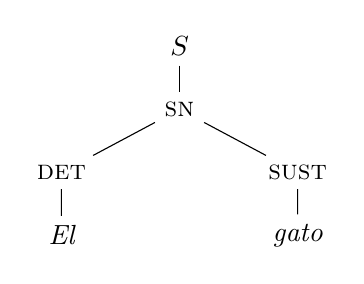
\begin{tikzpicture}[level/.style={sibling distance = 6cm/#1,
    level distance = 0.8cm},scale=1.0, transform shape]
\node  {$S$}
child
{
    node {\textsc{sn}}
    child
    {
        node {\textsc{det}}
        child {
            node {\em El}
        }
    }
    child{
        node {\textsc{sust}}
        child {
            node {\em gato}
        }
    }
};
\end{tikzpicture}
    \caption{Árbol de derivación de \textit{El gato}}
    \label{intro:arbol}
\end{figure}

\begin{definicion}[CFG]
Formalmente, una {\em gramática libre de contexto} $\gram$ se define como una 4-tupla $\gram = (N, \Sigma, S, R)$, donde:
\begin{itemize}
    \item $N$: conjunto de símbolos no terminales
    \item $\Sigma$: conjunto de símbolos terminales $(\Sigma \cap N = \emptyset)$
    \item $S$: símbolo inicial $(S \in N)$
    \item $R : N \times (N \cup \Sigma)^{\ast} $: conjunto de reglas o producciones \sergio{verificar santi notación}
\end{itemize}

\end{definicion}

\begin{definicion}[Derivación Directa]
Sean $r \in R : (A \to \beta)$ una producción, y $\beta, \gamma \in (N \cup \Sigma)^{\ast}$ cualquier par de cadenas, decimos que $\alpha A \gamma$ {\em deriva directamente} a $\alpha \beta \gamma$ y lo notamos $\alpha A \gamma \Rightarrow \alpha \beta \gamma$
\end{definicion}

\begin{definicion}[Derivación]
Sean $\alpha_1, \alpha_2 \cdots \alpha_m \in (N \cup \Sigma)^{\ast}$, $m \geq 1$, tal que:
$$
\alpha_1 \Rightarrow \alpha_2\quad,\quad \alpha_2 \Rightarrow \alpha_3\quad,\quad \cdots\quad,\quad \alpha_{m-1} \Rightarrow \alpha_m
$$
decimos que $\alpha_1$ deriva $\alpha_m$ y lo notamos como $\alpha_1 \xRightarrow{\ast} \alpha_m$
\end{definicion}

\begin{definicion}[Lenguaje libre de contexto]
Sea $\gram$ una gramática libre de contexto. Definimos al lenguaje de la gramática $L_\gram = \{w \mid w \in \Sigma^{\ast}, S \xRightarrow{\ast} w \}$ como el conjunto de los símbolos terminales que pueden derivarse a partir del símbolo inicial. A su vez, un lenguaje $L$ es libre de contexto si existe una gramática libre de contexto $\gram$ tal que $L = L_\gram$.
\end{definicion}


\subsection{Gramática libre de contexto probabilística}\label{sub:pcfg}

Las gramáticas libres de contexto probabilísticas (PCFG, por sus siglas en inglés) \cite{booth1969probabilistic} son uno de los formalismos más simples y a la vez poderosos para construir modelos probabilísticos de la estructura sintáctica de un lenguaje. Pueden entenderse como una extensión de las gramáticas libres de contexto donde cada regla tiene asociada una probabilidad que indica cuán probable es su uso para la derivación de un símbolo.

\begin{definicion}[PCFG]
Una gramática libre de contexto probabilística $\gram$ se define como una 5-tupla $\gram = (N, \Sigma, S, R, P)$, donde:
\begin{itemize}
    \item $N, \Sigma, S, R$ tienen el mismo significado que en las gramáticas libres de contextos
    \item $P : R \times [0,1]$ es la distribución de probabilidad $P$ que expresa la probabilidad de derivación de cada regla $P(\beta \mid A)$ con $(A \to \beta) \in R$.
\end{itemize}
Por lo tanto, si consideramos todas las posibles derivaciones de un símbolo, la suma de sus probabilidades debe ser 1:
$$
\sum_{\beta} P (A \to \beta) = 1.
$$
\end{definicion}
El modelo de PCFG permite asignar probabilidades a las derivaciones (o árboles de derivación) y a las palabras del lenguaje, lo cual lo convierten en una herramienta interesante para el modelado de lenguajes y su aplicación en distintos problemas como el reconocimiento de voz, traducciones automáticas, verificación y corrección de oraciones, etc.

Es importante destacar que todo árbol de derivación $T$ describe una única cadena $c$. Es decir, $P(T,c) = P(T) P(c\mid T) = P(T)$. La probabilidad de un árbol de derivación $P(T)$ está definida como el producto de la probabilidad de todas las reglas $\alpha_{i} \Rightarrow \beta_i$ usadas en su derivación, es decir,
$$
P(T) = \prod_{\alpha \Rightarrow \beta\in T} P(\alpha \Rightarrow \beta).
$$

Las suposiciones del modelo, por lo tanto, implican que la probabilidad de un subárbol no depende en qué lugar de la cadena ocurre ni tampoco depende de ningún símbolo terminal o no-terminal por fuera del subárbol.

Para calcular la probabilidad de una cadena $c$ alcanza entonces con sumar la probabilidad de todos los árboles de derivación que pueden producir esa cadena:
%
$$
P(c) = \sum_{\substack{T\ \mid \text{ árbol de}\\\text{derivación} \\  \text{de } S \xRightarrow{\ast} c }}   P (T).
$$



\subsection{Semántica}\label{sub:semantica}

Los modelos probabilísticos de \lot permiten realizar inferencia sobre un espacio de hipótesis estructurado gramaticalmente~\cite{goodman2008rational}. Cada propuesta de \lot suele formalizarse mediante una gramática libre de contexto $ \gram $ que define las funciones o programas válidos que se pueden generar, como en cualquier otro lenguaje de programación. Sin embargo, para representar conceptos es necesario unir estos elementos sintácticos con el conocimiento semántico que tenemos del mundo. Es decir, el programa (o árbol de derivación de $ \gram $) debe interpretarse o ejecutarse de acuerdo con una semántica determinada para obtener una descripción del concepto en la tarea cognitiva en cuestión. Esta tesis se basa fuertemente en que los \lot no sólo tienen una sintaxis definida por su gramática, sino que tienen una semántica determinada que les permite representar nuestro entendimiento del mundo.

En nuestro ejemplo de Logo, podíamos combinar las operaciones como `mover'', ``lápiz arriba'', ``lápiz abajo'' o ``rotar'' en distintos programas (o expresiones), pero sólo al ser evaluados es cuando estos programas pueden transmitir las distintas formas o conceptos que el lenguaje busca modelar.



Para un segundo ejemplo más concreto, consideremos la gramática del lenguaje Python. Una palabra de dicho lenguaje será cualquier programa válido. Así, una expresión (programa) como 
%
\begin{verbatim}
    s=""
    for i in range(30):
        s=s+"10"
    print(s)
\end{verbatim}
%
tendrá como semántica lo que este programa devuelve o imprime por pantalla, en este caso, la cadena
$$
01010101010101010101010101010101010101010101010101010101010.
$$

Es fundamental distinguir entre el espacio sintáctico de las descripciones o programas, que viene dado por una gramática $\gram$ por un lado, y el espacio de los objetos descriptos $\+O$ por otro. Aunque los dos espacios tendrán algún tipo de representación simbólica, pueden estar construidos sobre alfabetos distintos. Dada una gramática $\gram$ y un objeto a representar $x$ perteneciente al lenguaje definido por $\gram$, usaremos la notación $\sem{x}_\gram\in\+O$ para referirnos a la semántica de $x$ asignada por $\gram$ (cuando la gramática subyacente quede clara del contexto, lo notaremos simplemente $\sem{x}$). La naturaleza de $x$ dependerá, desde luego, del problema a analizar. 

La semántica $\sem{x}_\gram$ debe ser {\em formal}, esto es, con un significado matemático preciso único. La semántica de $x$ vendrá dada por los elementos que la componen, de acuerdo al árbol sintáctico que $\gram$ le asigne a $x$. Así, las definiciones de semántica $\sem{x}_\gram$ tendrán la forma de definiciones recursivas, que utilizan definiciones $\sem{y}_\gram$, donde $y$ es una subestructura de $x$ que dependerá, de $\gram$.

% En esta tesis, utilizaremos definiciones formales para representar la semántica de nuestras gramáticas $\gram$ donde el dominio serán los programas válidos de $\gram$ y el codominio los objetos a representar en cada tarea. 


La división entre $\gram$ y $\+O$ es central en esta tesis.
En la parte~\ref{parte:secuencias}, trabajaremos con los lenguajes \gramgeo y \grambin en el rol de $\gram$, que permiten modelar el espacio $\+O$ de secuencias en un octágono y secuencias binarias, respectivamente. En la parte~\ref{parte:conceptos}, utilizaremos la lógica proposicional \grambool como gramática de descripción $\gram$ para representar el espacio $\+O$ de conceptos booleanos. 


%Un lenguaje que describe conceptos (como formas) también proporciona una noción natural de su complejidad~\cite{kolmogorov1968three}. Un concepto es simple, relativo a ese lenguaje, cuando puede describirse mediante un programa corto. Por el contrario, es complejo cuando todas sus descripciones requieren una larga secuencia de instrucciones. Por ejemplo, en el caso del lenguaje Logo, un cuadrado puede simplemente instruirse como un bucle de cuatro desplazamientos seguidos de rotaciones de 90 grados. En este lenguaje, el icono de un rostro se implementará mediante un programa mucho más largo y, por lo tanto, será más complejo. Sin embargo, este concepto sería más sencillo cuando se describiera en un lenguaje en el que el icono de un rostro (o los símbolos de nariz, boca, etc.) estén disponibles como primitivos en el lenguaje.

%En el dominio de los conceptos booleanos, se estudió una amplia gama de variedades lógicas de conceptos en ~\cite{feldman2003simplicity}, revelando una ley sorprendentemente simple: la dificultad subjetiva de un concepto booleano para un aprendiz humano es directamente proporcional a la longitud del programa compatible más corto en el lenguaje de la lógica proposicional (es decir, variables booleanas combinadas con los operadores \textit{and}, \textit {or} y \textit{not}). Este resultado puede sugerir que el LoT humano está equipado con reglas y símbolos similares a los que se encuentran en la lógica proposicional. De hecho, la correlación entre la dificultad subjetiva de los conceptos y su complejidad se ha utilizado como vehículo general para estudiar el LoT humano en varios dominios ~\cite{piantadosi2016logical, leeuwenberg1971perceptual, amalric2017language, romano2018, lupyan2007language}. Aunque a menudo está implícito, la estrategia general es (\textit{1)} asumir un idioma; (\textit{2)} encontrar el programa compatible más corto para algunos conceptos en ese idioma; (\textit{3)} comparar la duración de estos programas con la dificultad subjetiva de los conceptos; y finalmente (\textit{4)} repetir este proceso para varios idiomas dentro de un universo de posibles candidatos y elegir el idioma que mejor se ajuste en \textit{(3)}. Como se mencionó anteriormente, la longitud del programa depende de las primitivas del lenguaje en el que está escrito este programa, por lo que diferentes lenguajes hacen diferentes predicciones.



%\section{Teoría algorítmica de la información}

%\intro{mandar a intro}{
%Un enfoque más formal para la estimación de la complejidad de los patrones, conocido como \textit{complejidad algorítmica}, \textit{complejidad del tamaño del programa} o \textit{complejidad de Kolmogorov} (CK), fue propuesto por Kolmogorov~\cite{kolmogorov1965three}, Chaitin~\cite{chaitin1969length} y Solomonof~\cite{solomonoff1964formal}, en el marco de la \textit{teoría algorítmica de la información}. Estos matemáticos definieron a la complejidad de una secuencia como la longitud del programa computacional más corto capaz de producirlo. Estrictamente hablando, la complejidad algorítmica se define en relación un lenguaje descriptivo (o lenguaje de programación). Cuando este lenguaje es Turing completo, lo que significa que se puede simular cualquier otra máquina de Turing en él, hablamos de CK universal o CK simplemente. Sin embargo, cuando el lenguaje de codificación tiene un poder expresivo reducido (es decir, cuando es una máquina específica en lugar de una máquina universal), la complejidad algorítmica se puede calcular y utilizar como una medida subjetiva de complejidad~\cite{romano2013language}\sergio{nosotros}. Recientemente, se propuso una aproximación a CK utilizando el \textit{teorema de codificación}, que relaciona la complejidad algorítmica de una secuencia con la probabilidad de que una máquina universal produzca esa secuencia~\cite{f43,f44,f45,f46}. La propuesta proporciona una medida de complejidad algorítmica para un gran conjunto de secuencias cortas. Esta propuesta se presentó como la mejor aproximación de “una medida final de aleatoriedad” y puede reproducir los sesgos observados cuando se les pide a los individuos que juzguen la aleatoriedad de los patrones o que produzcan patrones aleatorios~\cite{f44,f45}.
%}

%Como se indicó anteriormente, una propuesta estrictamente relacionada con la CK es que los sujetos humanos comprimen las secuencias internamente, no necesariamente usando un conjunto de instrucciones de un lenguaje universal, sino usando una variedad de primitivas similares a las de una computadora tales como bucles y otras rutinas que forman un \textit{lenguaje del pensamiento} (LoT, por sus siglas en inglés) \santi{Repe} interno específico~\cite{fodor1975language} lo suficientemente fuerte para describir cualquier secuencia del dominio, pero no tan complejo como el de una Máquina de Turing universal y, por lo tanto, lo suficientemente débil como para permitir que la complejidad pueda ser computada de manera exacta. Dicho lenguaje permitiría la combinación de primitivas simples en patrones complejos de encajes o reglas recursivas. Los modelos de LoT se han propuesto muy temprano~\cite{f33}. Simon y Kotovsky~\cite{f48} utilizaron conceptos como ``igual'', ``siguiente'' (en el alfabeto) y la capacidad de recorrer una serie para construir una representación formal de la memoria humana para secuencias de letras (por ejemplo, ``cadaeafa...''). Del mismo modo, Restle~\cite{f37} utilizó las operaciones ``repetir'', ``transposición'' y ``reflexión''. También se utilizaron lenguajes similares basados en repeticiones con variaciones para codificar figuras geométricas lineales y formas 2D y 3D más elaboradas~\cite{f33,leeuwenberg1971perceptual}. Más recientemente, se han utilizado con éxito propuestas similares para estudiar diferentes aspectos del aprendizaje humano, en particular el aprendizaje de conceptos~\cite{feldman2000minimization,f51, piantadosi2012bootstrapping,piantadosi2016four,f54}. \santi{media tesis es sobre esto. Referenciar a los capítulos correspondientes} Se ha mostrado que la complejidad Booleana, es decir, la longitud de la expresión lógica más corta que captura el concepto (una noción estrechamente relacionada con CK) captura el comportamiento humano en el aprendizaje de conceptos lógicos~\cite{feldman2000minimization,feldman2003simplicity}.

%\paragraph{Ubicar 2}

%En pocas palabras, la suposición es que para minimizar la carga de memoria, los participantes comprimen mentalmente la estructura de la secuencia utilizando el lenguaje formal propuesto.\santi{Esta es la visión de Mariano, la que dice que usamos este lenguaje... Para mí, es simplemente que este lenguaje lo puede explicar y que nuestra cabeza podría estar usando otro. Tal vez valga la pena una pequeña digresión sobre esto en las conclusiones.} El uso de un número mínimo de operaciones primitivas y la selección de la representación más corta, están en sintonía con el principio de simplicidad (propuesto como un componente esencial del aprendizaje) el cual define que las hipótesis más simples son las más favorecidas~\cite{f32,feldman2003simplicity}.


\section{Teoría Algorítmica de la Información}


Cuando vemos las palabras de 60 bits
\begin{align*}
\sigma_1 &= 01010101010101010101010101010101010101010101010101010101010,\\
\sigma_2 &= 00101000101000101000101000101000101000101000101000101000101,\\
\sigma_3 &= 01111100100011111001010111100011110100000100100011010101010,
\end{align*}
tenemos la sensación de que  $\sigma_2$ y  $\sigma_3$
son {\em más difíciles} o {\em más complejas} que $\sigma_1$, y quizá que $\sigma_2$ es más simple que $\sigma_3$. Sin embargo, en términos de
teoría de la medida, cada una es igual de probable, si provienen de una fuente que emite bits 
con probabilidad uniforme. 
La intuición es que las palabras sencillas tienen patrones reconocibles (como $\sigma_1$, y, aunque más oculto, $\sigma_2$) mientras que las más complejas no (o al menos no tienen patrones simples). Lo cierto es que $\sigma_3$ fue generada tirando una moneda y anotando 0 si salía cara y 1 si salía ceca. Nuestra intuición también nos dice que lo más probable es que una palabra generada mediante este procedimiento no tenga patrones reconocibles.

Entender por qué
algunas secuencias parecen aleatorias o complejas mientras que otras no, es una cuestión
profunda y fundamental. Desde principios del siglo {\small XX} se
empezó a pensar en este problema. Pero cómo transformar nuestra
intuición de `lo complejo' en una definición matemática, y cómo calibrar esta noción, no fue una tarea fácil. 
Al final, las definiciones que se
encontraron terminaron estando todas muy relacionadas con los métodos efectivos y con la 
teoría de la computación.

% La {\em teoría de largo de programa} define una noción de
% complejidad que clasifica las cadenas de 0s y 1s según la longitud
% del programa más corto que las computa. Esta complejidad se llama
% {\em complejidad de Kolmogorov}. Las cadenas más complejas son
% aquellas que requieren un programa esencialmente de igual longitud
% que la cadena misma, y las más sencillas son las que admiten un
% programa sustancialmente más corto. 

La Teoría Algorítmica de la Información, también
conocida como Teoría de Largo de Programa fue iniciada
independientemente en la década del 60 por Kolmogorov~\cite{kolmogorov1965three},
Solomonoff~\cite{solomonoff1964formal} y Chaitin~\cite{chaitin1969length}. 
Esta teoría define una
noción de complejidad de cada palabra teniendo en cuenta la longitud
del programa más corto que computa esa palabra. Así, los programas
son vistos como {\em descripciones algorítmicas} de palabras. De
entre todas las descripciones de una palabra podemos tomar la que
tiene menor longitud como una medida de su complejidad. Una palabra
$\sigma$ es simple, es decir, tiene baja complejidad, si su
complejidad es sustancialmente menor que la longitud de $\sigma$; y
una palabra es compleja si su descripción algorítmica es tan larga
como la longitud misma de $\sigma$. La gran mayoría
de las palabras tiene complejidad alta. La función que asocia a cada
palabra $\sigma$ la longitud del programa más corto que devuelve
$\sigma$ como salida (cuando es ejecutado en una cierta máquina
universal de referencia) se llama {\em complejidad de Kolmogorov} o
{\em complejidad de largo de programa}.

Debe
observarse que en esta definición --todavía informal-- 
de complejidad de Kolmogorov hay
un lenguaje de descripción subyacente. La teoría algorítmica de la información
adopta a los lenguajes de programación como lenguajes de descripción. Sin embargo, 
hay que notar que una definición en la misma dirección puede aplicarse para 
otros objetos en el rol de las palabras binarias (por ejemplo, conjuntos de valuaciones 
Booleanas) y otros lenguajes de descripción en el rol de lenguajes de programación
(por ejemplo, fórmulas de la lógica proposicional). En todo caso, es fundamental
que los lenguajes de descripción tengan una semántica formal para evitar paradojas
como la de Berry, que propone definir $n$ como el primer número natural que no sea 
descriptible con menos de 90 caracteres (por definición la descripción más corta de $n$ debe tener al menos 91 letras, y sin embargo su definición ``el primer número natural que no sea descriptible con menos de cincuenta caracteres'' evidentemente lo describe y tiene 83 caracteres).

% Desde el punto de 
% vista teórico, la riqueza de la Complejidad de Kolmogorov, y su intrincada conexión con la teoría de la computabilidad,
% aparece cuando el lenguaje de programación subyacente es 
% Turing-completo, 
% es decir, es capaz de definir cualquier función parcial
% computable. En la teoría, los lenguajes de programación se
% formalizan con máquinas de Turing y los lenguajes Turing-completos
% como máquinas universales. 
% Cuando el dominio de los programas (máquinas) es libre de prefijos (es decir, no hay dos programas
% que terminan en dónde uno es una extensión propia del otro)
% hablamos de complejidad de Kolmogorov {\em libre de prefijos}
% (denotada con $K$) y cuando no se impone ninguna restricción en
% el dominio, hablamos de complejidad de Kolmogorov plana (denotada
% con $C$). La necesidad de trabajar con dominios libres de prefijos es
% técnica y está vinculada con la utilidad de la complejidad de Kolmogorov 
% para definir nociones de aleatoriedad.
% Esta noción de complejidad es absoluta, pues si bien existe una
% complejidad distinta por cada máquina universal subyacente, todas
% estas son iguales salvo una constante aditiva~\cite{C94,li2013introduction}.

% A continuación veremos las definiciones formales de la Complejidad de Kolmogorov y de los
% principales elementos de la Teoría Algorítmica de la Información.

% Los orígenes del estudio de la aleatoriedad algorítmica se remontan
% a los trabajos de von Mises de principios del siglo {\small XX}
%~\cite{M19}, en dónde argumentaba que las secuencias aleatorias deben
% tener ciertas propiedades de estocasticidad desde el punto de vista
% de la teoría clásica de la probabilidad.

% Intuitivamente una secuencia es aleatoria cuando carece de
% estructura o regularidad, en otras palabras, cuando no tiene
% patrones reconocibles. Uno querría definir a las secuencias
% aleatorias como aquellas que  son indistinguibles del resultado de
% arrojar infinitas veces una moneda y anotar $0$ si sale cara o $1$
% si sale ceca. Así, las secuencias
% $$
% 00000000000000000000\dots \mbox{\quad o \quad }
% 10101010101010101010\dots
% $$
% no parecen aleatorias porque se pueden reconocer marcados patrones.
% En cambio, uno siente que una secuencia como
% $$
% 10010111010111100101\dots
% $$
% es aleatoria porque es difícil reconocer patrones. Las
% clarificaciones de precisamente qué constituye lo aleatorio fueron
% hechas recién pasada la mitad del siglo {\small XX}.

% Martin-L\"of~\cite{M66} introdujo una noción de aleatoriedad basado
% en tests estadísticos. La idea es que una secuencia aleatoria
% debería pasar todo posible test estadístico razonable. Martin-L\"of
% formaliza esta noción de {\em test estadístico razonable} como un
% tipo particular de conjuntos efectivos de medida $0$. Su propuesta
% es que una secuencia es aleatoria cuando evita (es decir, logra
% escapar de) todos esos conjuntos efectivos de medida $0$.

% Independientemente, Chaitin~\cite{C76b} introdujo la noción de
% aleatoriedad en términos de la complejidad de Kolmogorov (en
% realidad, de una variante de esa complejidad que se denomina
% complejidad {\em libre de prefijos}): las secuencias
% Chaitin-aleatorias son aquellas cuyos segmentos iniciales son {\em
% incompresibles}. Es decir, la complejidad de Kolmogorov de los
% primeros $n$ dígitos de la secuencia es mayor que $n$ menos una
% constante fija.


% Es interesante el hecho de que la idea de {\em procedimiento
% efectivo} está involucrada en todas las definiciones de aleatoriedad. 

\subsection{Complejidad de Kolmogorov} \label{INTRO:KOLMOGOROV}
% \widesanti{Introducir la noción formal. Empezar por $K_M$, con $M$ una máquina específica. Luego la $K_U$, con $U$ universal. Dar la versión plana y la libre de prefijos (puesto que esa es la que se usa para el coding theorem). Dar el coding theorem sin demo, solo enunciado.}


% \widesanti{Podés retomar los ejemplos de $\sigma_1$, $\sigma_2$, $\sigma_3$ de más arriba y explicar que programas cortos los generan. O podés exagerarlos a más bits. Esto da idea de la diferencia entre la descripción y lo descripto (aunque es cierto que la tesis es sobre aprendizaje con POCOS datos...) Para los programas, alcanza con un pseudo código o incluso descripción informal, pero dado que es una tesis en computación, también podés usar un lenguaje verdadero, Python, ponele. Podés también poner alguna otra cadena, $\sigma_4$ en donde haga falta anidar loops, porque eso es importante para el cap 2. Por ejemplo, 000111000 1 000111000 1 000111000}


% \widesanti{Esto que sigue es parte de mi tesis. Podés simplemente traducirlo y dejarlo tal cual. 
% Ojo que hay cosas de más... y muchos comandos latex :P}


% In this section we introduce the plain and \pfree \kolcomp and we
% mention some known results and standard notation that will be used
% repeatedly in the rest of this thesis. Some other important
% results will be introduced when necessary.

En esta sección introducimos la definición formal de \kolcomp y mencionamos algunos resultados que se relacionan con el desarrollo de esta tesis. Suponemos que el lector está familiarizado con los elementos básicos de la teoría de la computación, en particular con las máquinas de Turing. Para más información sobre estos temas, se pueden consultar textos clásicos como~\cite{O99,R87,S87}.

Como ya dijimos, en la Teoría Algorítmica de la Información, los programas son vistos como descripciones algorítmicas de palabras. Decimos que un programa $\pra$
{\em $\M$-describe} una palabra $\sta$ cuando, al ser ejecutado en una máquina $\M$, produce $\sta$ como salida. En general
hay más de un programa que describe la salida $\sta$.
La idea de la \kolcomp introducida en~\cite{kolmogorov1965three,solomonoff1964formal,chaitin1975theory} es tomar la longitud de la descripción más corta como una medida de la complejidad de la palabra. Si $\pra$ es un programa de una máquina de Turing, notamos $\len{\pra}$ a la {\em longitud} de $\pra$, es decir, a la cantidad de símbolos que tiene. Por $\words$ notamos al conjunto de palabras finitas formadas por los símbolos $0$ y $1$. Las definiciones que siguen fijan en $\words$ al alfabeto de programas y al de descripciones por simplicidad. Sin embargo, todas estas definiciones siguen teniendo sentido cuando los alfabetos de los programas son distintos a los de las palabras que describen; el único requerimiento es que ambos alfabetos sean finitos.
%
\begin{definicion}[\kolcomp]\label{intro:def:plainC}
$\CM\colon\words \to \nat$, la {\em 
\kolcomp con respecto a la máquina $\M$}, se define como
$$
\CM(\sta)=
    \begin{cases}
    \min \{\len{\pra}\colon \M(\pra)=\sta \} & \textrm{si $\sta$ está en el rango de $\M$};\\
    \infty & \textrm{caso contrario.}
    \end{cases}
$$
\end{definicion}


% \widesanti{acá hablar solo de la complejidad plana. Decir que la complejidad relativa a una máquina universal es la más chica entre todas las complejidades (salvo cte aditiva). Decir que para algunas máquinas particulares la complejidad es una función computable y dar un ejemplo simple - podria ser una máquina que dado n representando un número en binario, devuelve 0000... n veces; o una máquina que sencillamente copia la entrada en la salida. Decir algo sobre el counting como está acá 

% https://www.dropbox.com/s/w95pz1euie8a39r/Li-Vitanyi.pdf?dl=0

% en Def 2.2.1 y párrafo siguiente (pag 116)

% Tal vez podemos decir que la def de Kolmogorov complexity induce la idea de MDL. 

% No hablar nada de prefix machines o prefix complexity en la intro. Sacar lo de Craft Chaitin y lo de oráculos.

% Pasar la def. de prefix machines, prefix complexity y coding thm al cap 3
% }


\begin{definicion}[\Optity]\label{intro:def:optimal}
\index{Turing!machine!universal@\opt} $\U$ es una máquina de Turing {\em \opt}  si y solo si
$$
(\forall e)(\exists c_e)(\forall \pra)(\exists \prb_{e,\pra})\,
[\U(\prb_{e,\pra})=\T_e(\pra) \ \wedge \len{\prb_{e,\pra}}\leq
\len{\pra}+c_e],
$$
donde $\T_0,\T_1,\T_2,\dots$ es una enumeración de todas las máquinas de Turing.
\end{definicion}

% When working with oracles, $\U$ will be \opt if it may simulate
% {\em any} other machine with {\em any} oracle, so it is {\em
% universally universal}. In the case of an \pfree \opt machine,
% $\U^A$ will be \pfree for all $A\subseteq\nat$.

% In general we use the same letter $\U$ for denoting both a
% classical \opt machine and a \pfree \opt machine; it will always
% be clear from the context which one we refer to. In~\cite{chaitin1975theory}
% Chaitin called these machines {\em optimal universal}, because
% they permit us to define the \kolcomp in an {\em optimal} way:


Las máquinas universales existen y son aquellas que permiten `simular' cualquier otra máquina. Análogamente, un lenguaje de programación es {\em Turing-completo} si permite definir cualquier función parcial computable. Python, C o Haskell son lenguajes Turing-completos. Los lenguajes Turing-completos inducen una definición de máquina universal. Por simplicidad, tomemos como alfabeto de programas el código ASCII y supongamos que $\U$ es la máquina que interpreta programas en Python. El siguiente programa 
\begin{verbatim}
    s=""
    for i in range(30):
        s=s+"10"
    print(s)
\end{verbatim}
describe la cadena $\sigma_1$ descripta más arriba. Este programa tiene longitud 44, de modo que $\CU(\sta_1)\leq 44$. Por otro lado, el siguiente programa
\begin{verbatim}
    s=""
    for i in range(30):
        s=s+"0"
        if i%3==0:
            s=s+"0"
        else:
            s=s+"1"
    print(s)
\end{verbatim}
tiene longitud 82 y describe a la secuencia $\sigma_2$ y por lo tanto $\CU(\sta_2)\leq 82$. Finalmente, el programa
\begin{verbatim}
    print("001111100100011111001010111
    100011110100000100100011010101010")
\end{verbatim}
tiene longitud 69 y por lo tanto $\CU(\sta_3)\leq 69$. Notar que en todas las menciones a $\CU$ en los ejemplos anteriores consideramos cotas superiores; efectivamente, no estamos seguros de que los programas que describimos sean los minimales.

Extendamos ahora las secuencias $\sigma_1$, $\sigma_2$ y $\sigma_3$ a $\sigma_1'$, $\sigma_2'$ y $\sigma_3'$ respectivamente, con 120 bits en lugar de 60. Tendremos descripciones de la misma longitud para $\sigma_1'$ y $\sigma_2'$ (basta reemplazar `30' por `60' en el código. Sin embargo, la mejor descripción que nos viene a la mente para $\sigma_3'$ es un programa que sencillamente escriba $\sigma_3'$ textualmente, que tiene cerca de 120 símbolos:
\begin{verbatim}
    print("001111100100011111001010111
    1000111101000001001000110101010101
    1101111111001001011110000011110001
    0110101101100110001110011")
\end{verbatim}
Un resultado fundamental de la Teoría Algorítmica de la Información es que la complejidad de Kolmogorov relativa a una máquina universal no es computable. Sin embargo, si suponemos que $\sigma_3'$ fue generada al azar, entonces la teoría indica que con alta probabilidad, $\CU(\sigma_3)$ será cercana a la longitud de la cadena descripta, es decir, cercana a 120.

% Observar que el argumento anterior no varía su esencia si consideramos un alfabeto binario para el conjunto de programas, como indica la teoría. En efecto, cada símbolo usado para definir un programa de Python podría ser transformado en una palabra de 7 bits mediante el código ASCII, por ejemplo. Así, tendríamos que multiplicar por 7 las cotas a la complejidad que mencionamos más arriba.


Decimos que una cadena $\sta$ es $c$-compleja con respecto a $\M$ si $\CM(\sta)\geq |\sta|-c$. Por un simple argumento de conteo sobre programas sobre un alfabeto binario (para otros alfabetos, el resultado es similar), se puede ver que para cualquier máquina $\M$, la cantidad de cadenas $\sta$ de longitud $n$ que son $c$-complejas con respecto a $\M$ es como mínimo $2^n-2^{n-c}+1$. Entonces hay como mínimo 1 cadena de longitud $n$ que es 0-compleja, como mínimo la mitad de las cadenas de longitud $n$ son 1-complejas, por lo menos tres cuartos de las de las cadenas de longitud $n$ son 2-complejas. En general, de las $2^n$ cadenas de longitud $n$, la parte $(1-1/2^c)$ son $c$-complejas.

% Siguiendo con el ejemplo de la máquina universal sobre el lenguaje Python, observemos que la cantidad de programas de tamaño a lo sumo $n$ es 
% $$
% \sum_{k=0}^n r^k=\frac{1-r^{n+1}}{1-r}
% $$
% donde $r$ es la cantidad de elementos del alfabeto de programas --en el caso de ASCII, será $r=2^7=128$.

Como dijimos antes, la complejidad de Kolmogorov relativa a una máquina universal (o a un lenguaje Turing-completo, como Python en el ejemplo anterior) no es computable. Sin embargo, para lenguajes que no son Turing-completos, diseñados con un propósito específico de describir ciertos tipos de objetos, la complejidad asociada se podría volver computable. En esta tesis se explota en repetidas ocasiones este hecho fundamental.

Terminamos esta sección con un resultado fundamental de la teoría:
%
\begin{teorema}[Invariancia]\label{intro:thm:invariance}
\index{Invariance Theorem} Si $\U$ es una máquina de Turing \opt entonces para toda máquina de Turing $\M$ hay una constante $c$ tal que para todo
$\CU(\sta)\leq \CM(\sta)+c$.
\end{teorema}
%
Entonces para cualesquiera dos máquinas universales $\U$ y $\V$, la
\kolcomp con respecto a $\U$ y a $\V$ es la misma salvo una constante aditiva, es decir, hay una constante  $c$ tal que 
$\abs{\CU(\sta)-\CV(\sta)}\leq c$ para cualquier palabra $\sta\in\words$. Así, la complejidad de Kolmogorov pasa a ser una noción absoluta, si se acepta una variación hasta la constante $c$. 

La riqueza de la Teoría de la Información Algorítmica en relación a nociones de aleatoriedad y vínculos con la Teoría de la Computabilidad se da cuando analizamos la complejidad de Kolmogorov relativa una máquina universal/lenguaje Turing-completo --cualquiera de ellos, gracias al teorema anterior. En esta tesis se estudia la complejidad de Kolmogorov relativa a lenguajes específicos, no universales, suficientemente expresivos como para describir distintos aspectos del objeto de estudio, pero suficientemente simples como para lograr una noción de complejidad que resulte computable.


% Of
% course the same is true for classical machines and $\C$. If there
% is no need to refer to the underlying \opt machine $\U$, one just
% writes \glossary{$\K$}$\K$ for $\KU$ and \glossary{$\C$}$\C$ for
% $\CU$. In this way, $\K$ and $\C$ become an {\em absolute} measure
% of the complexity of the strings.

% To illustrate some useful application of the Invariance Theorem,
% let us see some upper bounds for $\K$ and $\C$. Imagine a
% classical machine $\M$ that reads the input $\sta$ and writes
% $\sta$ as its own output. Then $\CM(\sta)=\len{\sta}$ for all
% $\sta\in\words$ and by the Invariance
% Theorem~\ref{intro:thm:invariance} this shows that for all $\sta$,
% $\C(\sta)\leq \len{\sta}+c$ for some constant $c$. With \pfree
% machines the situation is a bit different because the machine has
% to discover by itself where the end of the input is. Suppose $\U$
% is any \opt \pfree machine and suppose $\pra_\sta$ is a minimal
% $\U$-description of $\len{\sta}$. This just means that
% $\U(\pra_\sta)=\len{\sta}$ and $\len{\pra_\sta}=\K(\len{\sta})$.
% Then there is a \pfree machine $\N$ that with input
% $\pra_\sta\sta$ can do the following: fist simulate $\U$ step by
% step. Each time $\U$ asks for reading one more bit, $\N$ obeys and
% reads from its own input. Eventually $\U$ will read the whole
% $\pra_\sta$ and will terminate with $\U(\pra_\sta)=\len{\sta}$ as
% output. Now $\N$ (which is still running) knows that exactly
% $\len{\sta}$ more bits need to be read from the input. So $\N$
% reads $\len{\sta}$ bits from the input and recovers $\sta$.
% Afterwards, $\N$ writes $\sta$ in the output and terminates. This
% shows that $\N(\pra_\sta\sta)=\sta$. Of course, if the input is
% wrong, the computation may go wrong, for example $\N$ can try to
% read beyond the end of the input and then crashes. However, when
% the input is of the form $\pra_\sta\sta$, $\N$ always outputs
% $\sta$. By the invariance Theorem \ref{intro:thm:invariance} this
% shows that $\K(\sta)\leq \len{\pra_\sta\sta} + d =
% \K(\len{\sta})+\len{\sta}+d$ for some constant $d$. These upper
% bounds on $\C$ and $\K$ will be repeatedly used in the thesis. We
% will also use that for any $n$ there is a string $\sta$ of length
% $n$ such that $\K(\sta)\geq n$. This is true because there are at
% most $2^n-1$ programs of length less than $n$ but $2^n$ strings of
% length $n$. The same holds for $\C$. In fact,
% Chaitin~\cite{chaitin1975theory,C87b} showed that there is a constant $c$ such
% that for all $d\in\nat$ and all $n$
% $$
% \size{\{ \sta \colon \len{\sta}=n \wedge \K(\sta)\leq n + \K(n)-d
% \}} \leq 2^{n-d+c}
% $$
% This result is usually called \index{Counting Theorem}Counting\santi{estos resultados de 'counting' pueden ser interesantes porque justifican algo que decimos en el cap 2. Buscar mi comentario con ***}
% Theorem, tells us that only a small fraction of all the strings of
% length $n$ have \pfree \kolcomp below $n+\K(n)-d$, when we take
% $d$ much bigger than $c$.
% Observe that if we let $d=n-b$, we obtain
% $$
% \size{\{ \sta \colon \len{\sta}=n \wedge \K(\sta)\leq \K(n)+b
% \}} \leq 2^{b+c}
% $$
% and this last upper bound depends on $b$ and $c$, but not on $n$.

% As we explained in the last paragraph, one way to bound the
% \kolcomp is to explicitly design specific machines, like $\M$ or
% $\N$ and explain their behavior. Another powerful method to
% implicitly build \pfree machines and upper bound the \pfree
% \kolcomp is via a Kraft-Chaitin set. This method consists of an
% effective interpretation of an inequality of Kraft~\cite{K49}:

%\begin{definicion}[Kraft-Chaitin set]\label{intro:KCset}
%\index{Kraft-Chaitin} A \ce\ set
%$$
%W=\{\pair{n_0}{\sta_0}, \pair{n_1}{\sta_1},
%\pair{n_2}{\sta_2},\dots\},
%$$
%where $n_i\in\nat$ and $\sta_i\in \words$, is a {\em %Kraft-Chaitin
%set} if $\wt{W}\leq 1$, where \glossary{$\wt{W}$}$\wt{W}=
%\sum_{i\in\nat} 2^{-n_i}$ is the {\em weight} of $W$. The %pairs
%enumerated into such a set $W$ are called {\em axioms}.
%\end{definicion}

%The Kraft-Chaitin Theorem can be found in Levin's
%Thesis~\cite{L71} and in~\cite{levin1974laws}, Schnorr also included a
%version of it in~\cite{S73} and Chaitin~\cite{chaitin1975theory} gave the first
%proof explicitly for \pfree \kolcomp. This theorem states that
%from a Kraft-Chaitin set $W$ like the one described in the above
%Definition~\ref{intro:KCset}, we can effectively obtain a \pfree
%machine $\M$ such that for each $i$ there is a $\pra_i$ of length
%$n_i$ with $\M(\pra_i)\downarrow=\sta_i$, and $\M(\prb)\uparrow$
%unless $\prb=\pra_i$ for some~$i$. Observe that the machine $\M$
%is built in an implicit way: we only need to specify the lengths
%of the programs we want. In particular, the Kraft-Chaitin Theorem
%states that there is a constant $c$ such that for all $i$,
%$\K(\sta_i)\leq\min\{m\colon\pair{m}{\sta_i}\in W\}+c$.



\subsection{Longitud mínima de descripción}


Para cada fenómeno siempre puede haber un número grande, posiblemente infinito, de explicaciones. Como vimos en  \S\ref{sub:semantica}, en un modelo de \lot este espacio está formalizado por la gramática $\gram$ que define las hipótesis válidas y el espacio de objetos $\+O$ que interpreta esas hipótesis en descripciones sobre los objetos a explicar. 

Una vez definido el espacio de hipótesis es importante definir un mecanismo de selección entre ellas. Uno de los principios más populares es el de la navaja de Ockham que postula que debe elegirse la hipótesis más simple entre todas las posibles explicaciones de un fenómeno. Este principio de selección de hipótesis fue formalizado por Rissanen \cite{rissanen1978modeling} y Wallace \cite{wallace1968information} en el método de longitud de descripción mínima (MDL por sus siglas en inglés) el cual postula que dado un objeto y una enumeración de explicaciones, la mejor explicación es la que minimiza la suma del tamaño en bits de la gramática $\gram$ y del tamaño en bits de la descripción del objeto $o \in \gram$. En términos de la complejidad de Kolmogorov, el principio ideal de MDL seleccionará dentro de la hipótesis $H$ que explican a $o$, la que minimiza $K(H) + K(o|H)$. Para mayor información sobre modelos ideales y prácticos de MDL, puede referirse a \cite{grunwald2007minimum,li2013introduction}.

En nuestro trabajo seleccionaremos descripciones dentro de una misma gramática, por lo cual, debemos definir sólo cómo calcular el tamaño de los programas definidos por $\gram$. A cada hipótesis / programa $x$ del lenguaje definido por $\gram$ le asignaremos un {\em tamaño}, notado $|x|$, que será un número natural. En términos generales, la idea es que contará la cantidad de símbolos de $x$, aunque la definición precisa podría dar más peso a ciertos símbolos por sobre otros. Es importante observar que el tamaño de un objeto $x$ es independiente de su semántica, en tanto es una propiedad de una descripción y no del objeto descripto.

En analogía con la complejidad de Kolmogorov de la Definición~\ref{intro:def:plainC} definimos la {\em longitud mínima de descripción} relativa a $\gram$ como la función $\mdl{\gram}:\+O\to\nat$ definida de esta forma:
%
\begin{equation}\label{eqn:mdl}
\mdl{\gram}(o)\eqdef\min\{|x|\mid x\in\gram,\sem{x}_{\gram}=o\}.
\end{equation}
%
Así, $\mdl{\gram}(o)$ será el tamaño de la descripción más corta que tenga $o$ entre las expresiones de $\gram$. Trabajaremos siempre con objetos que tengan al menos una descripción en $\gram$. Esta noción de complejidad sí utiliza la semántica asociada a $\gram$. Desde luego, la definición precisa dependerá de los lenguajes estudiados y del espacio de objetos que se quieran modelar: la definición \eqref{eqn:mdl} es simplemente un marco que será instanciado en distintos lenguajes y semánticas a lo largo de la tesis --incluso en algunos casos, como en las gramáticas de la Parte \ref{parte:secuencias}, la semántica dependerá también de `puntos de evaluación'. Es importante notar que la definición \eqref{eqn:mdl} no es otra cosa más que la complejidad de Kolmogorov relativa a una máquina de Turing específica, posiblemente Turing-incompleta. De hecho, para las investigaciones que siguen, los lenguajes propuestos estarán específicamente diseñados para entender una pequeña porción del mundo, aquella que queremos modelar, y los lenguajes serán siempre Turing-incompletos. Una propiedad necesaria será que la función $\mdl{\gram}$ sea computable, e incluso implementable eficientemente.





\section{Inferencia Bayesiana}
 
Otro mecanismo de selección de hipótesis comúnmente utilizado es la inferencia bayesiana. En este caso, a diferencia de MDL, las predicciones que realizaremos no se basarán en la mejor explicación, sino que utilizará todas las explicaciones posibles sobre un objeto pesadas por su probabilidad de ocurrencia. 

A diferencia de la estadística clásica o frecuentista que construye métodos estadísticos para decidir la probabilidad de obtener ciertos datos bajo ciertas asunciones mínimas, la inferencia bayesiana trata de asignar probabilidades a las hipótesis en sí utilizando toda la información disponible.

Para conocer la probabilidad de una hipótesis $h$ dado un conjunto de datos $d$, la inferencia bayesiana utiliza simplemente el Teorema de Bayes:

$$
P(h|d) = \frac{P(d|h) * p(h)}{P(d)}
$$

En estos casos se conoce a $P(h|d)$ como la probabilidad a posteriori dado los datos $d$ y esta reescritura en función de $P(d|h)$,$P(h)$ y $P(d)$ nos permitirá a lo largo de esta tesis elegir y comprar distintas hipótesis a partir de los datos.

A $P(h)$ se la conoce como probabilidad a priori, y representa la probabilidad de una hipótesis antes de cualquier observación. Esta distribución denota de manera explícita el conocimiento que se asume sobre las hipótesis antes de realizar la inferencia. Las distribuciones a priori se pueden crear a partir de experimentos o conocimientos previos, a partir de la decisión subjetiva de un experimentador, generando un equilibrio entre los resultados cuando no hay información disponible y/o utilizar una de las distribuciones a priori conjugadas para simplifica el cálculo de la distribución a posteriori. En esta tesis, utilizaremos algunas distribuciones a priori conjugadas como la Dirichlet y definiremos la probabilidad a priori de las hipótesis de una gramática $\gram$ a partir de la probabilidad de su árbol de derivación según lo visto en \S\ref{sub:pcfg}.

La distribución $P(d)$ se la conoce como distribución marginal de los datos, y es la probabilidad de observar los datos bajo todas las hipótesis. El cálculo de esta probabilidad implica integrar todas las posibles hipótesis, lo cual no siempre es posible, pero es importante notar que al comparar la probabilidad de dos hipótesis, este valor es constante y se puede prescindir de su cálculo. 

Por último, a $P(d|h)$ se la conoce como la función de verosimilitud y es la probabilidad de que se observen los datos $d$ cuando la hipótesis $h$ es verdadera. Para esta probabilidad es fundamental en nuestra tesis la definición de semántica en \S\ref{sub:semantica} que describe los objetos $\+O$. Una regla simple será definir que $P(d|h)$ es 1 cuando la hipótesis explique los datos y 0 cuando no, es decir, será 1 si $\sem{h}_\gram = d$.

Muchas veces la cantidad de hipótesis a integrar hacen que no sea eficiente o plausible calcular la distribución entera de probabilidad de todas las hipótesis de manera exacta. Para esto, existen diversos mecanismos de aproximación de la distribución de probabilidad. Uno de los más sencillos es utilizar la hipótesis más probable, conocido comúnmente como máximo a posteriori (MAP). Es decir, $P(d|H) \approx P(d|h_{MAP})$. En el caso que $H$ contenga sólo hipótesis determinísticas, es decir, donde $P(d|h_i)$ es 1 si $h_i$ explica $d$ y $0$ sino, entonces $h_{MAP}$ es la hipótesis más probable. En este caso $MAP$ elige como hipótesis más simple a la más probable mientras que $MDL$ lo hace con la hipótesis más pequeña en términos de su tamaño.

\sergio{No sé si este párrafo suma o no. }

%\section{Sin ubicar:}
%"The infite use of finite means" (Humboldt's sobre el lenguaje)

%1) How does abstract knowledge guide learning and inference from sparse data?
%Bayesian inference in probabilistic generative models

%2) What form does that knowledge take, across different domains and tasks?
%Probabilities defined over richly structured symbolic representations: spaces, graphs, grammars, logical predicates

%3) How is that knowledge itself constructed / updated / validated?
%Hierarchical models, transfer learning, herramientas papers


%La mayoría de los estudios de LoT se han centrado en el aspecto compositivo del lenguaje, que se ha modelado dentro de un~\cite{tenenbaum2011grow} bayesiano o un marco~\cite{marie2016, goldsmith2002probabilistic, romano2013language, goldsmith2001unsupervised} de longitud mínima de descripción (MDL).

%El método común es definir una gramática con un conjunto de producciones basadas en operaciones que son intuitivas para los investigadores y luego estudiar cómo diferentes procesos de inferencia coinciden con patrones regulares en el aprendizaje humano. Un estudio reciente~\cite{piantadosi2016logical} pone el foco en el proceso de cómo elegir empíricamente el conjunto de producciones y cómo diferentes definiciones de LoT pueden crear diferentes patrones de aprendizaje. 

%\subsection{Ciencia Cognitiva Bayesiana}
%\label{INTRO:BAYES}
%\subsubsection{Rational analysis y plot}

%Aunque el estudio actual se basa en el uso de un lenguaje fijo, con reglas y pesos asociados, alguna evidencia sugiere que una mejor descripción del comportamiento se puede lograr incorporando un componente probabilístico al modelado. Este enfoque, defendido por~\cite{piantadosi2016four} bajo el término lenguaje de pensamiento probabilístico (pLoT), consiste en utilizar inferencia probabilística bayesiana para estimar la probabilidad de la existencia de algún conjunto de reglas (un lenguaje formal propuesto), dada los datos observados. Se ha demostrado que es especialmente eficaz para modelar el aprendizaje de conceptos,por ejemplo, replicando los patrones de errores a lo largo del aprendizaje~\cite{goodman2008rational,piantadosi2012bootstrapping,piantadosi2016logical}. Este enfoque también se adoptó para investigar cómo los seres humanos evalúan la aleatoriedad en su entorno. Los sesgos humanos en los juicios subjetivos de aleatoriedad~\cite{f114,f115} podrían explicarse asumiendo que la representación de la aleatoriedad resulta de una inferencia estadística sobre los procesos que generaron la secuencia, es decir, una estimación de la probabilidad de que un proceso regular dado lo produjo~\cite{f21}. Un buen ajuste al comportamiento humano fue obtenido sin utilizar toda la potencia de las máquinas de Turing, sino simplemente autómatas de estado finito con una pila, que son capaces de reconocer la repetición, la alternancia o la simetría~\cite{f18,f117}. Por lo tanto, a pesar de las diferencias fundamentales (en particular, los lenguajes deterministas versus probabilísticos), la teoría pLOT comparte con nuestro enfoque la necesidad de considerar tipos similares de operaciones primitivas. Dados los fuertes vínculos entre aleatoriedad y complejidad subjetivas, podemos esperar razonablemente que nuestro lenguaje formal también puede predecir si un patrón se percibe como aleatorio o no; esta posibilidad permanece para ser probado en trabajos futuros.

%Como se mencionó anteriormente, el enfoque pLOT permite encontrar los conceptos y reglas más probables en un espacio de hipótesis estructurado gramaticalmente que contiene varios candidatos utilizando la inferencia bayesiana, parece ser un enfoque muy prometedor para ese propósito~\cite{goodman2008rational,piantadosi2016four,romano2018bayesian}. 